%                                                                 aa.dem
% AA vers. 9.1, LaTeX class for Astronomy & Astrophysics
%\documentclass[referee]{aa}
\documentclass{aa}
%
\usepackage[varg]{txfonts}
\usepackage{graphicx}
\usepackage{float}
\usepackage{natbib}
\bibpunct{(}{)}{;}{a}{}{,}
\usepackage[colorlinks,linkcolor=blue,urlcolor=blue,citecolor=blue]{hyperref}
\usepackage{threeparttablex}
\usepackage{longtable}
\usepackage{lscape}
\usepackage{bm}
\usepackage{verbatim}
\usepackage{makecell}
\usepackage{caption}
\usepackage{subcaption}
\usepackage{multirow}
\usepackage{booktabs}
\usepackage{threeparttable}
\usepackage{colortbl}
\usepackage{xcolor}
%
%
\begin{document}

\title{X-ray Properties of Hickson Compact Groups in COSMOS-Web to $z \sim 3.8$: Hot Gas in Dense, Dynamically Evolving Systems (Paper~II)}

\author{Ghassem Gozaliasl\inst{1,2}\thanks{e-mail: ghassem.gozaliasl@aalto.fi}
  \and
  Günther Hasinger\inst{3}
  \and
  [Co-authors TBD]}

\institute{Department of Computer Science, Aalto University, PO Box 15400, 00076, Espoo, Finland\\
\and
Department of Physics, University of Helsinki, Gustaf H\"{a}llstr\"{o}m katu 2, 00560 Helsinki, Finland\\
\and
[Hasinger affiliation TBD]}

\date{[Date TBD]}

\abstract{
[PLACEHOLDER --- to be written when results are finalised.]

We present a comprehensive X-ray analysis of 912 Hickson Compact Groups (CW-HCG) identified within the COSMOS-Web footprint (Hasinger et al., in preparation) using deep Chandra and XMM-Newton observations combined with JWST NIRCam imaging. This is the second paper in a series characterizing the hot intragroup medium (IGM) of COSMOS-Web galaxy groups; Paper~I \citep{Gozaliasl2026a} presented the same uniform X-ray analysis pipeline applied to the full COSMOS-Web group catalog (CW-All; 1,678 systems). Applying a detection threshold of SNR~$\geq 2.0$, we detect X-ray emission from 305 CW-HCG groups (33.4\%), a slightly higher fraction than the CW-All rate of 29.6\%, which we interpret as [TBD --- enhanced core surface brightness? selection effects?]. Stacking across nine redshift bins yields high-significance composite detections out to $z \sim 3.8$, revealing [TBD --- evolution description]. Direct comparison with CW-All stacked luminosities shows [TBD]. These results constrain the role of group compactness and enhanced galaxy interactions in shaping the hot intragroup medium, with implications for understanding compact group evolution and eventual merging into single massive galaxies.
}{galaxies: evolution -- galaxies: groups: compact -- galaxies: groups: X-ray -- galaxies: high-redshift -- surveys}{}{}{}

\maketitle

%-------------------------------------------------------------------

\section{Introduction}

Hickson Compact Groups (HCGs) represent one of the densest known galaxy environments outside of cluster cores. Originally catalogued by \citet{Hickson1982} from photographic plates of the local universe, they are defined by strict criteria requiring at least four member galaxies within a 3~mag window of the brightest member, high surface density, and isolation from comparable-brightness field galaxies. The resulting systems --- typically containing 4--5 galaxies in projected separations of tens to hundreds of kpc --- are thought to represent either a distinct evolutionary track toward complete galaxy merging, or a transient dynamical state in the early assembly of normal groups \citep{MendesDeOliveira1994}.

The X-ray properties of HCGs have been studied extensively in the local universe. \citet{Ponman1996} established that $\sim$75\% of the original \citet{Hickson1982} catalog show diffuse X-ray emission, with luminosities and temperatures broadly consistent with normal groups at the same halo mass. However, a subset of compact groups exhibit anomalously low X-ray luminosities at fixed optical richness, suggesting that tidal stripping, AGN feedback, or incomplete virialization may reduce the hot gas content \citep{Mulchaey2000,Osmond2004}. At higher redshifts, compact group samples have been identified through a range of methods --- overdensity criteria, photometric redshift slices, AMICO-based detection applied to deep photometric surveys --- but their X-ray properties as a population remain largely unconstrained beyond $z \sim 0.5$.

The identification of 912 COSMOS-Web Hickson Compact Groups (CW-HCG) over $0.45~\mathrm{deg}^2$ to $z \sim 3.8$ (Hasinger et al., in preparation) provides an unprecedented opportunity to study compact group X-ray evolution across more than 12~Gyr of cosmic history. The depth and resolution of JWST NIRCam, combined with the legacy X-ray coverage of the COSMOS field from Chandra and XMM-Newton, enable both individual detections and stacking analyses that constrain ensemble hot gas properties across the full redshift range of the survey.

In this paper (Paper~II of the series), we present the X-ray analysis of the CW-HCG sample using the identical pipeline applied to CW-All in Paper~I \citep{Gozaliasl2026a}, enabling a direct, controlled comparison between the general group population and compact group systems at the same redshifts and survey depths. Our specific goals are: (i) to quantify the CW-HCG X-ray detection rate and how it compares with CW-All at fixed redshift and richness; (ii) to measure luminosities, temperatures, and halo masses for individually detected compact groups; (iii) to recover ensemble X-ray properties via stacking for systems below the detection threshold; and (iv) to test whether compact group environments enhance or suppress hot gas emission relative to the general group population, and whether this depends on redshift.

The paper is organized as follows. Section~\ref{sec:data} describes the CW-HCG catalog and the X-ray data. Section~\ref{sec:analysis} summarizes the analysis methodology (identical to Paper~I; we refer the reader there for full details). Section~\ref{sec:results} presents the detection statistics, individual measurements, and stacking results. Section~\ref{sec:comparison} compares CW-HCG with CW-All. Section~\ref{sec:discussion} discusses the implications for compact group evolution. Section~\ref{sec:conclusions} summarizes our conclusions. Throughout we adopt a Planck 2018 flat $\Lambda$CDM cosmology \citep{Aghanim2020} with $H_0 = 67.4$~km~s$^{-1}$~Mpc$^{-1}$ and $\Omega_{\rm m} = 0.315$.

\section{Data}
\label{sec:data}

\subsection{The COSMOS-Web Hickson Compact Group Catalog}

The CW-HCG sample is presented in Hasinger et al.\ (in preparation). [PLACEHOLDER: describe the selection algorithm, criteria applied to COSMOS-Web galaxies, redshift range, richness distribution, comparison with Hickson 1982 original criteria, any photometric vs.\ spectroscopic confirmation statistics.]

The catalog contains 912 compact groups spanning $0.12 \lesssim z \lesssim 3.83$ with a median redshift of $z \approx 0.97$. [Add: distribution of group sizes, member counts, projected separations, stellar masses, BGG properties.]

For the X-ray analysis we use all 912 systems. We note that [TBD: any quality cuts, masking, or exclusions specific to CW-HCG not applied to CW-All].

\subsection{X-ray Data}

The X-ray data are identical to those used in Paper~I: the combined Chandra and XMM-Newton mosaic of the COSMOS field in the 0.5--2.0~keV band, covering $\sim 2~\mathrm{deg}^2$ with a flux limit of $3 \times 10^{-16}~\mathrm{erg~cm^{-2}~s^{-1}}$ \citep{Gozaliasl2019}. We refer the reader to Paper~I (Section~2.4) for a full description of the X-ray maps, their uncertainty images, and the point-source masking procedure.

\section{Analysis methodology}
\label{sec:analysis}

The X-ray analysis of CW-HCG is performed with the identical pipeline described in Paper~I (Section~3), including: adaptive aperture photometry (baseline 300~kpc aperture with refinement to $R_{500}$ for detections), redshift-binned median background cross-check, adaptive sigma clipping, two-pass detection with SNR~$\geq 2.0$ threshold, K-correction, and scaling relations for temperature and halo mass. We refer the reader to Paper~I for full methodological details and only note here any CW-HCG-specific choices.

[PLACEHOLDER: note any differences --- e.g., if CW-HCG required smaller minimum aperture due to projected compactness; any treatment of projected neighbours within the compact group itself.]

\section{Results}
\label{sec:results}

\subsection{X-ray detection statistics}

[PLACEHOLDER]

We detect X-ray emission from 305 of 912 CW-HCG groups (33.4\%) at SNR~$\geq 2.0$. Table~\ref{tab:detection_hcg} summarises the detection statistics and median physical properties of the detected subsample. [Compare with CW-All 29.6\%; discuss significance and possible drivers.]

\subsection{X-ray luminosity and the $L_{\rm X}$--redshift plane}

[PLACEHOLDER]

Figure~\ref{fig:LX_z_hcg} shows the rest-frame 0.5--2.0~keV luminosity as a function of redshift for all CW-HCG systems. Individual detections, 95\% upper limits for non-detections, and flagged upper limits follow the same convention as Figure~5 of Paper~I. Stacked median luminosities from Section~\ref{sec:stacking_hcg} are over-plotted.

\subsection{Halo masses}

[PLACEHOLDER]

Halo masses are derived from the same weak-lensing calibrated $M$--$L_{\rm X}$ scaling relation as in Paper~I \citep{Leauthaud2010}. Figure~\ref{fig:M200_hcg} shows $M_{200}^{L_{\rm X}}$ versus redshift for individually detected CW-HCG groups.

\subsection{Stacking analysis}
\label{sec:stacking_hcg}

[PLACEHOLDER]

Table~\ref{tab:stacking_hcg} lists the stacked CW-HCG ensemble measurements across nine redshift bins. Figure~\ref{fig:stacking_hcg} shows the stacked luminosities, fluxes, SNR, and $M_{200}^{L_{\rm X}}$ as a function of redshift, comparing all-group stacks (solid) with detection-only stacks (dashed).

\subsection{Radial surface-brightness profiles}

[PLACEHOLDER]

Stacked X-ray radial surface-brightness profiles for CW-HCG are shown in Figure~\ref{fig:profiles_hcg} for three representative redshift bins. [Discuss central peaking, PSF comparison, extended emission significance.]

\section{Comparison with the general group population (CW-All)}
\label{sec:comparison}

[PLACEHOLDER --- this section is the scientific heart of Paper II.]

\subsection{Detection rate comparison}

[PLACEHOLDER: CW-HCG 33.4\% vs.\ CW-All 29.6\%. Is this difference significant? Redshift-dependent? Richness-dependent?]

\subsection{Stacked luminosity comparison}

[PLACEHOLDER: Direct comparison of CW-HCG and CW-All stacked $L_{\rm X}$ at matched redshift bins. Figure~\ref{fig:comparison_stacks}. Discuss any excess/deficit and its physical interpretation.]

\subsection{Radial profile comparison}

[PLACEHOLDER: Are CW-HCG profiles more centrally concentrated? Extended emission fraction?]

\subsection{Scaling relation offsets}

[PLACEHOLDER: At fixed $M_{200}$ or richness, do compact groups sit on the same $L_{\rm X}$--$M$ or $L_{\rm X}$--$T$ relation as CW-All? Plot offset from the relation as a function of projected compactness or member separation.]

\section{Discussion}
\label{sec:discussion}

\subsection{Physical interpretation of compact group X-ray properties}

[PLACEHOLDER]

\subsection{Redshift evolution of the hot gas fraction in compact groups}

[PLACEHOLDER]

\subsection{Role of tidal interactions and enhanced merger rates}

[PLACEHOLDER]

\subsection{AGN contamination and feedback in compact group environments}

[PLACEHOLDER: Compact groups may have elevated AGN fractions; discuss contamination mitigation and any evidence for AGN-driven gas heating or expulsion.]

\section{Conclusions}
\label{sec:conclusions}

[PLACEHOLDER]

We have presented a uniform X-ray analysis of 912 COSMOS-Web Hickson Compact Groups spanning $0.12 \lesssim z \lesssim 3.83$, using the same Chandra+XMM-Newton mosaic and analysis pipeline applied to the full COSMOS-Web group sample in Paper~I \citep{Gozaliasl2026a}. Our main conclusions are:

\begin{enumerate}
  \item [TBD] Detection rate: 305/912 (33.4\%) at SNR~$\geq 2.0$.
  \item [TBD] Median detected $L_{\rm X}$, $T$, $M_{200}$ values.
  \item [TBD] Stacking results and redshift evolution.
  \item [TBD] Comparison with CW-All: similar/different luminosities, profile shapes.
  \item [TBD] Physical interpretation.
\end{enumerate}

\begin{appendix}

\section{Radial surface-brightness stacking and PSF tests for CW-HCG}

\subsection{Stacked profiles by redshift bin}

[PLACEHOLDER: same methodology as Appendix~A of Paper~I; present full set of CW-HCG profiles across all redshift bins.]

\subsection{Random-stack null tests}

[PLACEHOLDER]

\section{Individual compact group X-ray notes}

[PLACEHOLDER: notes on particularly interesting individual systems --- strongly detected compact groups, unusual morphologies, AGN hosts, etc.]

\end{appendix}

%-------------------------------------------------------------------

\begin{thebibliography}{}

\bibitem[Aghanim et al.(2020)]{Aghanim2020} Aghanim, N., Akrami, Y., Ashdown, M., et al.\ 2020, A\&A, 641, A6

\bibitem[Anderson et al.(2015)]{Anderson2015} Anderson, M.~E., Gaspari, M., White, S.~D.~M., Wang, W., \& Dai, X.\ 2015, MNRAS, 449, 3806

\bibitem[Bellagamba et al.(2018)]{Bellagamba2018} Bellagamba, F., Roncarelli, M., Maturi, M., \& Moscardini, L.\ 2018, MNRAS, 473, 5221

\bibitem[Casey et al.(2023)]{Casey2023} Casey, C.~M., Kartaltepe, J.~S., Drakos, N.~E., et al.\ 2023, ApJ, 954, 31

\bibitem[Civano et al.(2016)]{Civano2016} Civano, F., Marchesi, S., Comastri, A., et al.\ 2016, ApJ, 819, 62

\bibitem[Elvis et al.(2009)]{Elvis2009} Elvis, M., Civano, F., Vignali, C., et al.\ 2009, ApJS, 184, 158

\bibitem[Finoguenov et al.(2007)]{Finoguenov2007} Finoguenov, A., Guzzo, L., Hasinger, G., et al.\ 2007, ApJS, 172, 182

\bibitem[George et al.(2011)]{George2011} George, M.~R., Leauthaud, A., Bundy, K., et al.\ 2011, ApJ, 742, 125

\bibitem[Gozaliasl et al.(2016)]{Gozaliasl2016} Gozaliasl, G., Finoguenov, A., Khosroshahi, H.~G., et al.\ 2016, MNRAS, 458, 2762

\bibitem[Gozaliasl et al.(2019)]{Gozaliasl2019} Gozaliasl, G., Finoguenov, A., Tanaka, M., et al.\ 2019, MNRAS, 483, 3545

\bibitem[Gozaliasl et al.(2026a)]{Gozaliasl2026a} Gozaliasl, G., et al.\ 2026, A\&A, submitted (Paper~I)

\bibitem[Hasinger et al.(2007)]{Hasinger2007} Hasinger, G., Cappelluti, N., Brunner, H., et al.\ 2007, ApJS, 172, 29

\bibitem[Hasinger \& Others(in preparation)]{Hasinger2025} Hasinger, G., \& Others.\ in preparation

\bibitem[Hickson(1982)]{Hickson1982} Hickson, P.\ 1982, ApJ, 255, 382

\bibitem[Kettula et al.(2015)]{Kettula2015} Kettula, K., Giodini, S., van Uitert, E., et al.\ 2015, MNRAS, 451, 1460

\bibitem[Khostovan et al.(2025)]{Khostovan2025} Khostovan, A.~A., Kartaltepe, J.~S., Salvato, M., et al.\ 2025, arXiv:2503.00120

\bibitem[Leauthaud et al.(2010)]{Leauthaud2010} Leauthaud, A., Finoguenov, A., Kneib, J.-P., et al.\ 2010, ApJ, 709, 97

\bibitem[Lovisari et al.(2015)]{Lovisari2015} Lovisari, L., Reiprich, T.~H., \& Schellenberger, G.\ 2015, A\&A, 573, A118

\bibitem[Marini et al.(2024)]{Marini2024} Marini, I., Popesso, P., Lamer, G., et al.\ 2024, A\&A, 689, A7

\bibitem[Maturi et al.(2019)]{Maturi2019} Maturi, M., Bellagamba, F., Radovich, M., et al.\ 2019, MNRAS, 485, 498

\bibitem[Mendes de Oliveira \& Hickson(1994)]{MendesDeOliveira1994} Mendes de Oliveira, C. \& Hickson, P.\ 1994, ApJ, 427, 684

\bibitem[Mulchaey(2000)]{Mulchaey2000} Mulchaey, J.~S.\ 2000, ARA\&A, 38, 289

\bibitem[Navarro et al.(1997)]{Navarro1997} Navarro, J.~F., Frenk, C.~S., \& White, S.~D.~M.\ 1997, ApJ, 490, 493

\bibitem[Osmond \& Ponman(2004)]{Osmond2004} Osmond, J.~P.~F. \& Ponman, T.~J.\ 2004, MNRAS, 350, 1511

\bibitem[Planck Collaboration et al.(2013)]{PlanckCollaboration2013} Planck Collaboration, Ade, P.~A.~R., et al.\ 2013, A\&A, 557, A52

\bibitem[Ponman et al.(1996)]{Ponman1996} Ponman, T.~J., Bourner, P.~D.~J., \& Ebeling, H.\ 1996, in Roentgenstrahlung from the Universe, 357--360

\bibitem[Popesso et al.(2024)]{Popesso2024} Popesso, P., Biviano, A., Bulbul, E., et al.\ 2024, MNRAS, 527, 895

\bibitem[Popesso et al.(2025)]{Popesso2025} Popesso, P., et al.\ 2025, A\&A, in press

\bibitem[Robson \& Dav\'e(2023)]{Robson2023} Robson, D. \& Dav\'e, R.\ 2023, MNRAS, 518, 5826

\bibitem[Shuntov et al.(2025)]{Shuntov2025} Shuntov, M., Akins, H.~B., Paquereau, L., et al.\ 2025, arXiv:2506.03243

\bibitem[Springel et al.(2005)]{Springel2005} Springel, V., White, S.~D.~M., Jenkins, A., et al.\ 2005, Nature, 435, 629

\bibitem[Sun et al.(2009)]{Sun2009} Sun, M., Voit, G.~M., Donahue, M., et al.\ 2009, ApJ, 693, 1142

\bibitem[Toni et al.(2024)]{Toni2024} Toni, G., Gozaliasl, G., Maturi, M., et al.\ 2024, A\&A, 697, A197

\bibitem[Toni et al.(2025)]{Toni2025} Toni, G., Maturi, M., Finoguenov, A., Moscardini, L., \& Castignani, G.\ 2024, A\&A, 697, A197

\bibitem[Wang et al.(2025)]{Wang2025} Wang, Q., Bogdan, \'A., Schellenberger, G., et al.\ 2025, Nature [arXiv:2601.19978]

\bibitem[White \& Rees(1978)]{White1978} White, S.~D.~M. \& Rees, M.~J.\ 1978, MNRAS, 183, 341

\bibitem[Willis et al.(2020)]{Willis2020} Willis, J.~P., Pacaud, F., Clerc, N., et al.\ 2020, A\&A, 638, A6

\end{thebibliography}

%-------------------------------------------------------------------
% FIGURES (placeholders — insert actual figure files when available)
%-------------------------------------------------------------------

\begin{figure}
\centering
%\includegraphics[width=\columnwidth]{figures/redshift_distribution_hcg}
\caption{[PLACEHOLDER] Redshift distribution of the CW-HCG sample (N=912, orange). The CW-All distribution (N=1678, blue, from Paper~I) is overlaid for comparison. Both samples peak at $z \sim 1$--1.5; CW-HCG has a slightly lower median ($z \approx 0.97$) compared to CW-All ($z \approx 1.1$). Panel~(b): X-ray detection rate as a function of redshift for CW-HCG (orange) and CW-All (blue dashed).}
\label{fig:redshift_dist_hcg}
\end{figure}

\begin{table}
\caption{Detection summary for the CW-HCG sample (SNR $\geq 2.0$). CW-All statistics from Paper~I are listed for direct comparison. Median properties are computed for the detected subsample.}
\label{tab:detection_hcg}
\centering
\begin{tabular}{lrrrcccr}
\hline\hline
Catalog & $N_{\rm tot}$ & $N_{\rm det}$ & Det.\ (\%) & Med.\ flux & Med.\ $\log L_{\rm X}$ & Med.\ $z$ & Med.\ $M_{200}$ \\
 & & & & (erg cm$^{-2}$ s$^{-1}$) & (erg s$^{-1}$) & & ($M_{\odot}$) \\
\hline
CW-HCG & 912  & 305 & 33.4 & $1.16\times10^{-15}$ & 42.88 & 0.97 & $2.82\times10^{13}$ \\
CW-All$^{a}$  & 1678 & 497 & 29.6 & $1.09\times10^{-15}$ & 42.97 & 1.10 & $2.88\times10^{13}$ \\
\hline
\end{tabular}
\tablefoot{$^{a}$ CW-All statistics reproduced from Paper~I \citep{Gozaliasl2026a} for comparison.}
\end{table}

\begin{figure*}
\centering
%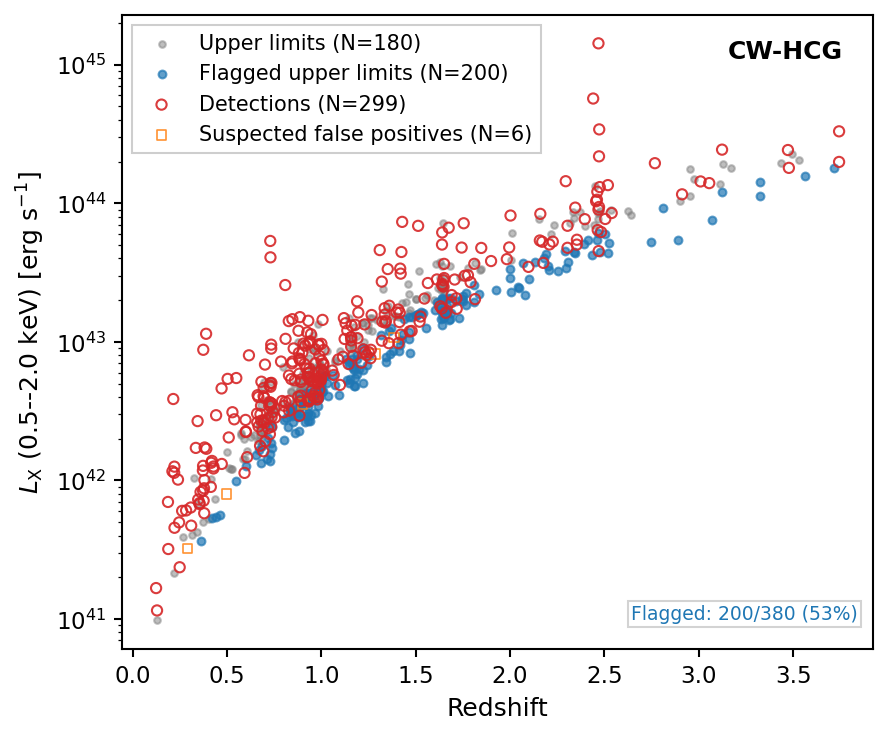
\includegraphics[width=0.8\textwidth]{figures/luminosity_redshift_cw_hcg}
\caption{[PLACEHOLDER] Rest-frame 0.5--2.0~keV luminosity $L_{\rm X}$ versus redshift for CW-HCG. Symbols follow the same convention as Figure~5 of Paper~I: large open circles = individual detections (SNR~$\geq 2.0$); grey points = non-detections with 95\% upper limits; blue points = flagged upper limits; orange squares = stacked median $L_{\rm X}$ per bin (Table~\ref{tab:stacking_hcg}).}
\label{fig:LX_z_hcg}
\end{figure*}

\begin{figure}
\centering
%\includegraphics[width=\columnwidth]{figures/m200_redshift_hcg}
\caption{[PLACEHOLDER] Halo mass $M_{200}^{L_{\rm X}}$ versus redshift for individually detected CW-HCG groups (orange squares), with CW-All detections (blue circles, from Paper~I) overlaid. Both samples span a similar mass range, probing group-scale halos at $M_{200} \sim 10^{13}$--$10^{14}~M_{\odot}$.}
\label{fig:M200_hcg}
\end{figure}

\begin{table*}
\caption{Stacked X-ray measurements for the CW-HCG sample across nine redshift bins. Fluxes are mean per-source values; uncertainties reflect bootstrap errors from 1000 resamplings.}
\label{tab:stacking_hcg}
\centering
\begin{tabular}{cccrrcrrr}
\hline\hline
$z_{\rm min}$ & $z_{\rm max}$ & $\langle z \rangle$ & $N_{\rm src}$ & SNR & \multicolumn{2}{c}{Flux (erg cm$^{-2}$ s$^{-1}$)} & \multicolumn{2}{c}{$L_{\rm X}$ (erg s$^{-1}$)} \\
 &  &  &  &  & Flux & $\sigma_F$ & $L_{\rm X}$ & $\sigma_L$ \\
\hline
0.25 & 0.50 & 0.38 &  51 &  6.53 & $2.62\times10^{-15}$ & $4.02\times10^{-16}$ & $1.64\times10^{42}$ & $2.51\times10^{41}$ \\
0.50 & 0.75 & 0.63 & 112 & 11.90 & $1.07\times10^{-15}$ & $8.95\times10^{-17}$ & $3.02\times10^{42}$ & $2.54\times10^{41}$ \\
0.75 & 1.00 & 0.88 & 223 & 14.07 & $6.23\times10^{-16}$ & $4.43\times10^{-17}$ & $3.82\times10^{42}$ & $2.72\times10^{41}$ \\
1.00 & 1.25 & 1.16 & 112 & 10.30 & $4.34\times10^{-16}$ & $4.21\times10^{-17}$ & $5.06\times10^{42}$ & $4.92\times10^{41}$ \\
1.25 & 1.50 & 1.39 &  88 &  6.01 & $4.94\times10^{-16}$ & $8.22\times10^{-17}$ & $9.61\times10^{42}$ & $1.60\times10^{42}$ \\
1.50 & 1.75 & 1.64 &  82 &  9.06 & $4.34\times10^{-16}$ & $4.79\times10^{-17}$ & $1.32\times10^{43}$ & $1.45\times10^{42}$ \\
1.75 & 2.00 & 1.88 &  23 &  3.66 & $4.51\times10^{-16}$ & $1.23\times10^{-16}$ & $1.80\times10^{43}$ & $4.93\times10^{42}$ \\
2.00 & 2.50 & 2.25 &  80 &  6.07 & $2.16\times10^{-16}$ & $3.56\times10^{-17}$ & $2.09\times10^{43}$ & $3.43\times10^{42}$ \\
2.50 & 3.80 & 3.15 &  39 &  6.44 & $3.98\times10^{-16}$ & $6.18\times10^{-17}$ & $6.18\times10^{43}$ & $9.61\times10^{42}$ \\
\hline
\end{tabular}
\tablefoot{$\log_{10} M_{200}$ values are included in the full electronic table (\texttt{xray\_catalog\_cwhcg.fits}).}
\end{table*}

\begin{figure*}
\centering
%\includegraphics[width=\textwidth]{figures/stacking_hcg_multi}
\caption{[PLACEHOLDER] Stacked X-ray properties of CW-HCG (orange) as a function of redshift, compared with CW-All (blue, from Paper~I). Solid lines: stacks from all groups per bin; dashed lines: stacks restricted to individually detected systems. From left to right: rest-frame $L_{\rm X}$, observed-frame flux, stacked SNR, and $M_{200}^{L_{\rm X}}$. [Discuss: similarities/differences between orange and blue curves.]}
\label{fig:stacking_hcg}
\end{figure*}

\begin{figure*}
\centering
%\includegraphics[width=0.32\textwidth]{figures/stacking_radial_profiles_hcg_z_0.05_0.25}
%\includegraphics[width=0.32\textwidth]{figures/stacking_radial_profiles_hcg_z_0.25_0.55}
%\includegraphics[width=0.32\textwidth]{figures/stacking_radial_profiles_hcg_z_0.55_0.95}
\caption{[PLACEHOLDER] Stacked 0.5--2~keV radial surface-brightness profiles for CW-HCG in three redshift bins. Blue points: stacked group profiles with $1\sigma$ uncertainties. Grey dotted: random-stack null tests. Orange dashed: analytic XMM-Newton PSF model normalised to the central surface brightness. [Compare profile width and central excess with Fig.~A.1 of Paper~I for CW-All.]}
\label{fig:profiles_hcg}
\end{figure*}

\begin{figure*}
\centering
%\includegraphics[width=\textwidth]{figures/comparison_stacks_cwall_vs_cwhcg}
\caption{[PLACEHOLDER] Direct comparison of stacked $L_{\rm X}$ (left) and $M_{200}^{L_{\rm X}}$ (right) between CW-HCG (orange squares) and CW-All (blue circles) as a function of median redshift. Shaded bands show $1\sigma$ bootstrap uncertainties. [Discuss: are compact groups brighter/fainter at fixed redshift? Does the offset evolve?]}
\label{fig:comparison_stacks}
\end{figure*}

\end{document}
